\documentclass[xetex,xcolor={table,usenames,dvipsnames}]{beamer}
\usepackage{ragged2e} % Ensure ragged2e is included
\usepackage{beamerthemesplit}
\usepackage[utf8]{inputenc}
\usepackage{ccicons}
\usepackage[T1]{fontenc}
\usepackage[english,french]{babel}
\usepackage{times}
\usepackage{tabularx}
\usepackage{dsfont}
\usepackage{textcomp}
\usepackage{amssymb}
\usepackage{graphicx}
\usepackage{bbding}
\usepackage{listings}
\definecolor{mygray}{rgb}{0.8,0.8,0.8}
\lstset{%
	basicstyle=\ttfamily,
	breaklines = true,
	backgroundcolor=\color{mygray},
}
\usepackage{realboxes}

\DeclareDocumentCommand{\clist}{v}{%
	\Colorbox{mygray}{\csname lstinline\endcsname!#1!}%
}
\usepackage[absolute,overlay]{textpos}
\usepackage[style=authoryear, maxbibnames=99, mincitenames=1, maxcitenames=2, backref=true, hyperref=true, dashed=false, firstinits=true, backend=bibtex, bibencoding=utf8, uniquename=false, uniquelist=false, natbib=true]{biblatex}
\renewcommand*{\bibfont}{\scriptsize}
\setbeamerfont{footnote}{size=\tiny}

% Remove quotation marks from titles
\DeclareFieldFormat[article,incollection,inproceedings,conference]{title}{#1} 

\usepackage{makecell}

\usepackage{capt-of}

\usepackage{xcolor}
\usepackage{shadowtext} 
% Define a custom color for lavender
\definecolor{lavender}{RGB}{230,230,250}
\definecolor{deepred}{RGB}{201,10,77}
\definecolor{deepblue}{RGB}{55,66,136}

\usepackage{hyperref}
 
 \hypersetup{
    colorlinks=true,      % Enable colored links
   linkcolor=violet,        % Color for internal links (sections, equations, etc.)
    citecolor=BlueViolet,      % Color for citations
    filecolor=magenta,    % Color for file links
    urlcolor=blue         % Color for URLs
}

\mode<presentation>
{
\usetheme{metropolis}


\setbeamercolor{header}{bg=MidnightBlue, fg=white} % Dark theme header
\setbeamercolor{progressdots}{fg=white} % Color for navigation dots

\setbeamertemplate{headline}{%
	% First row: Section Titles
	\begin{beamercolorbox}[wd=\paperwidth,ht=2.5ex,dp=1ex,center]{header}
		\textbf{\insertsectionnavigationhorizontal{\paperwidth}{}{}}
	\end{beamercolorbox}
	
	% Second row: Navigation Dots (one per frame under each section)
	\begin{beamercolorbox}[wd=\paperwidth,ht=1.5ex,dp=0ex,center]{progressdots}
		\hspace{5pt} % Adjust spacing
		\foreach \sec in \inserttotalsections { % Loop through sections
			\foreach \fr in {1,...,\insertsectionframe} { % Loop through frames in section
				\ifnum\fr=\insertframeinsection
				{\color{white}●} % Highlight current frame in section
				\else
				{\color{gray}○} % Other frames in section
				\fi
				\hspace{3pt} % Adjust spacing between dots
			}
			\hspace{10pt} % Space between sections
		}
	\end{beamercolorbox}
}

\setbeamertemplate{footline}{%
	\begin{beamercolorbox}[wd=\paperwidth,ht=2.5ex,dp=1ex,leftskip=3mm,rightskip=3mm]{footline}
		\hspace{3mm} \textbf{Ljudmila PETKOVI\'C} \hfill
		\textbf{\textsc{M2SOL034} : Automates et transducteurs à états finis $\cdot$ Unitex} \hfill
		\textbf{\today} \hspace{3mm}
	\end{beamercolorbox}%
}


\setbeamertemplate{headline}{%
	\begin{beamercolorbox}[wd=\paperwidth,ht=2ex,dp=1ex,center]{frametitle}
		\insertsectionnavigationhorizontal{\paperwidth}{}{}
	\end{beamercolorbox}%
}
\setbeamertemplate{footline}{%
	\begin{beamercolorbox}[wd=\paperwidth,ht=4ex,dp=1ex,leftskip=3mm,rightskip=3mm]{footline}
		\hspace{3mm} 
		\textcolor{gray}{\textbf{Ljudmila PETKOVI\'C}} \hfill
		\textcolor{gray}{\textbf{\textsc{M2SOL034} : Automates et transducteurs à états finis $\cdot$ Unitex}} \hfill 
		\textcolor{gray}{\textbf{\today}} \hspace{3mm}
		\textcolor{gray}{\textbf{\insertframenumber{} / \inserttotalframenumber}} \hspace{3mm} % Page number in bottom-right
	\end{beamercolorbox}%
	
	% Add the logo only if we're NOT on the title slide
	\ifnum\insertframenumber>0
	\begin{textblock*}{2.5cm}(\paperwidth-2cm,1\textheight) % Move slightly down and right
		
\includegraphics[width=1.2cm]{img/logo.png} % Adjusted logo size
	\end{textblock*}
	\fi
}









%\usecolortheme{beaver}
\usefonttheme{professionalfonts}
}







\usepackage{listings}

\lstset{ 
  language=C,                     % Set language
  basicstyle=\ttfamily\small,      % Set basic style to small monospaced font
  keywordstyle=\color{blue},       % Set keywords in blue
  commentstyle=\color{gray},       % Set comments in gray
  stringstyle=\color{red},         % Set strings in red
  numbers=left,                    % Line numbers on the left
  numberstyle=\tiny\color{gray},   % Style for line numbers
  stepnumber=1,                    % Line number step
  showstringspaces=false,          % Don't show spaces in strings
  tabsize=4,                       % Set tab size
  breaklines=true,                 % Break long lines
  captionpos=b                     % Caption position bottom
}

\usepackage[font=scriptsize,justification=centering]{caption}
\setbeamercolor{normal text}{fg=black,bg=black}
\setbeamercolor{frametitle}{fg=purple,bg=white}
\setbeamercolor{background canvas}{bg=white}
\setbeamercolor{title}{fg=purple}
\setbeamercolor{subtitle}{fg=purple}
\setbeamercolor{section in toc}{fg=purple}
\setbeamercolor{footline}{fg=purple,bg=white}
%\setbeamercolor{block title}{fg=purple,bg=white}
%\setbeamercolor{block body}{fg=white,bg=black}

\newcommand{\bolder}[1]{{\color{purple}\bfseries#1}}

% Set bullet points color to gold
\setbeamercolor{itemize item}{fg=violet}
\setbeamercolor{itemize subitem}{fg=violet}
\setbeamercolor{itemize subsubitem}{fg=violet}


\beamertemplatetransparentcovered
\beamerboxesdeclarecolorscheme{myalert}{red}{black!5!averagebackgroundcolor}
\beamerboxesdeclarecolorscheme{mybox}{blue}{black!5!averagebackgroundcolor}


%% Customize the colors for the footer
%\setbeamercolor{footline}{bg=white,fg=violet} % Set background to violet and text to white
%\setbeamercolor{footline title}{bg=white,fg=violet}
%\setbeamercolor{footline section}{bg=white,fg=violet}
%\setbeamercolor{footline page}{bg=white,fg=violet}
%
%% Customize the footer
%\setbeamertemplate{footline}{%
%  \leavevmode%
%  \hbox{%
%    \begin{beamercolorbox}[wd=.333\paperwidth,ht=2.25ex,dp=1ex,leftskip=3mm,rightskip=3mm,center]{footline title}%
%      \usebeamerfont{author in head/foot}\insertshorttitle
%    \end{beamercolorbox}%
%    \begin{beamercolorbox}[wd=.333\paperwidth,ht=2.25ex,dp=1ex,center]{footline section}%
%      \usebeamerfont{author in head/foot}\insertsection
%    \end{beamercolorbox}%
%    \begin{beamercolorbox}[wd=.333\paperwidth,ht=2.25ex,dp=1ex,right,center]{footline page}%
%      \usebeamerfont{author in head/foot}\insertframenumber{} / \inserttotalframenumber
%    \end{beamercolorbox}%
%  }%
%  \vskip0pt%
%}

\setbeamercolor{block title}{bg=violet,fg=white}
\setbeamercolor{block body}{bg=lavender,fg=black}


 \newcommand{\cf}{\textit{cf.} }
 \newcommand{\ie}{\textit{i.e.} }
 \newcommand{\ev}{espace vectoriel }
 \newcommand{\ssi}{si et seulement si }




\newcommand{\espc}[1]{\esp\left[ #1 \right]}

\newcommand{\defe}{\stackrel{\mbox{\begin{tiny}
 déf
 \end{tiny}}}{=}}
 \newcommand{\tend}[2]{\mathop{\longrightarrow}\limits_{#1\rightarrow #2}}

\newcommand{\rem}{\noindent\textbf{Remark : }}
\newcommand{\rems}{\textbf{Remarques: }}

\newcommand{\exs}{\textbf{Exemples: }}

\newcommand{\imp}[1]{\textbf{\textit{#1}}}


%\newtheorem{lem}{\textbf{Lemma}} 
%\newtheorem{theo}{\textbf{Theorem}} %[section]
%\newtheorem{prop}{\textbf{Proposition}}%[chapter]
%\newtheorem{coro}{\textbf{Corollary}}%[chapter]
%\newtheorem{hyp}{\textbf{Hypothesis}}
%\newtheorem{defi}{\textbf{Definition}}
%\newtheorem{pdefi}{\textbf{Proposition-D\'{e}finition}}

%\newenvironment{proof}[1][Proof : ]{\begin{trivlist}
%\item[\hskip \labelsep {\bfseries #1}]}{\hfill $\Box$\end{trivlist}}
%
%\newtheorem{lem}{\textbf{Lemme}} 
%\newtheorem{theo}{\textbf{Théorème}} %[section]
%\newtheorem{prop}{\textbf{Proposition}}%[chapter]
%\newtheorem{coro}{\textbf{Corollaire}}%[chapter]
%\newtheorem{hyp}{\textbf{Hypothèses}}
%\newtheorem{defi}{\textbf{Définition}}
%\newtheorem{pdefi}{\textbf{Proposition-D\'{e}finition}}
%\newtheorem{rmq}{\textbf{Remarque}} 

\usepackage{pgf,pgfarrows,pgfnodes,pgfautomata,pgfheaps,pgfshade}


%\font\bbfnt=msbm6
%\def\bbN{\mbox{\bbfnt N}}
%\def\bbR{\mbox{\bbfnt R}}
%\title{Champs aléatoires gaussiens}
%\author{Victor Rabiet}
%\institute{EMSE}
%\date[APSSE]{Présentation du 17 décembre 2015}

%===================================================
%===================================================
\usepackage{etoolbox} % Required for \apptocmd

% Make subitems smaller
\makeatletter
\patchcmd{\itemize}
{\def\makelabel}
{\setlength{\itemsep}{2pt} % Adjust spacing if needed
	\def\makelabel{\textbf{\scriptsize}}} % Change to \small, \footnotesize, or \scriptsize
{}
{}
\makeatother

% Make subsubitems even smaller
\makeatletter
\patchcmd{\itemize}
{\def\makelabel}
{\setlength{\itemsep}{1pt} % Adjust spacing
	\def\makelabel{\textbf{\tiny}}} % Use a smaller font size
{}
{}
\makeatother

% Change subitem bullets to circles
\setbeamertemplate{itemize subitem}{\raisebox{0.15em}{\scriptsize$\circ$}}

% Optionally, change subsubitem bullets to smaller circles
\setbeamertemplate{itemize subsubitem}{\raisebox{0.15em}{\tiny$\circ$}}


\addtobeamertemplate{frametitle}{}{%
\begin{textblock*}{2cm}(11.5cm,0.2cm) % Adjust position here

\end{textblock*}}


\addbibresource{bibliographie.bib}


\let\oldnocite\nocite
\makeatletter
\renewcommand*{\nocite}[1]{\oldnocite{#1}\Hy@backout{#1}}
\makeatother

\renewcommand*{\bibfont}{\footnotesize}

\DeclareCiteCommand{\cite}
{\usebibmacro{prenote}}
{\usebibmacro{citeindex}%
	\printtext[bibhyperref]{\usebibmacro{cite}}}
{\multicitedelim}
{\usebibmacro{postnote}}

\DeclareCiteCommand*{\cite}
{\usebibmacro{prenote}}
{\usebibmacro{citeindex}%
	\printtext[bibhyperref]{\usebibmacro{citeyear}}}
{\multicitedelim}
{\usebibmacro{postnote}}

\DeclareCiteCommand{\parencite}[\mkbibparens]
{\usebibmacro{prenote}}
{\usebibmacro{citeindex}%
	\printtext[bibhyperref]{\usebibmacro{cite}}}
{\multicitedelim}
{\usebibmacro{postnote}}

\DeclareCiteCommand*{\parencite}[\mkbibparens]
{\usebibmacro{prenote}}
{\usebibmacro{citeindex}%
	\printtext[bibhyperref]{\usebibmacro{citeyear}}}
{\multicitedelim}
{\usebibmacro{postnote}}

\DeclareCiteCommand{\footcite}[\mkbibfootnote]
{\usebibmacro{prenote}}
{\usebibmacro{citeindex}%
	\printtext[bibhyperref]{ \usebibmacro{cite}}}
{\multicitedelim}
{\usebibmacro{postnote}}

\DeclareCiteCommand{\footcitetext}[\mkbibfootnotetext]
{\usebibmacro{prenote}}
{\usebibmacro{citeindex}%
	\printtext[bibhyperref]{\usebibmacro{cite}}}
{\multicitedelim}
{\usebibmacro{postnote}}

%\DeclareCiteCommand{\textcite}
%  {\boolfalse{cbx:parens}}
%  {\usebibmacro{citeindex}%
	%   \printtext[bibhyperref]{\usebibmacro{textcite}}}
%  {\ifbool{cbx:parens}
	%     {\bibcloseparen\global\boolfalse{cbx:parens}}
	%     {}%
	%   \multicitedelim}
%  {\usebibmacro{textcite:postnote}}

%\DeclareCiteCommand{\textcite}
%{\usebibmacro{cite:init}%
%	\usebibmacro{prenote}}
%{\usebibmacro{citeindex}%
%	\printtext[bibhyperref]{\usebibmacro{textcite}}}
%{}
%{\printtext[bibhyperref]{\usebibmacro{textcite:postnote}}%
%	\usebibmacro{cite:post}}

%\DeclareCiteCommand{\textcite}
%{\usebibmacro{prenote}}
%{\printnames[final={\&}]{author} \bibhyperref{(\printfield{year})}}
%{\multicitedelim}
%{\usebibmacro{postnote}}


\usepackage{tikz}
\usetikzlibrary{automata, positioning, arrows}
\tikzset{
	->, % makes the edges directed
	>=stealth', % makes the arrow heads bold
	node distance=3cm, % specifies the minimum distance between two nodes. Change if necessary.
	every state/.style={thick, fill=gray!10}, % sets the properties for each ’state’ node
	initial text=$ $, % sets the text that appears on the start arrow
}
	
\DefineBibliographyStrings{french}{%
	backrefpage = {voir p\adddot},%
	backrefpages = {voir pp\adddot}%
}
\DeclareFieldFormat{pagerefformat}{\mkbibparens{{\color{red}\mkbibemph{#1}}}}
\renewbibmacro*{pageref}{%
	\iflistundef{pageref}
	{}
	{\printtext[pagerefformat]{%
			\ifnumgreater{\value{pageref}}{1}
			{\bibstring{backrefpages}\ppspace}
			{\bibstring{backrefpage}\ppspace}%
			\printlist[pageref][-\value{listtotal}]{pageref}}}}



\begin{document}


\title{{\large Corpus, ressources et linguistique outillée $\cdot$ \textsc{M2SOL034}}}
\subtitle{CM 4 : Automates et transducteurs à états finis $\cdot$ Unitex}
\author{\footnotesize{Ljudmila PETKOVI\'C}}
\institute{{\scriptsize Sorbonne Université\\Master \og{}Langue et Informatique\fg{} (\textsc{M1} ScLan)\\\textsc{UFR} Sociologie et Informatique pour les Sciences Humaines}\\~\\{\tiny Cours adapté de \textcite{fort}, de \textcite{nouvel} et de \textcite{tanguy}.}}
\date{\scriptsize{Semestre 2, 2024-2025\\\today}}




	\frame{\titlepage}

\section{Automates et transducteurs}


\begin{frame}{Automates finis}
	
	{	\scriptsize angl. \textit{\textbf{F}inite-\textbf{S}tate \textbf{A}utomata} }
	
	\begin{itemize}
		\item machine permettant de définir un langage
		\item capable d'indiquer si une chaîne fait partie ou non du langage
		\item chaîne entrée $\rightarrow$ [automate] $\rightarrow$ oui/non
	\end{itemize}


\end{frame}


\begin{frame}{États}
	Indiquent où en est l'analyse d'un mot.
	\vspace{5pt}
	\begin{table} % Wrapping inside a table environment
		\centering
		\begin{tabular}{c l}  
			% Column 1: TikZ Nodes
			\begin{minipage}{0.3\textwidth} % Minipage for TikZ
				\centering
				\tikz \node[state] (qi) {$q\textsubscript{i}$}; \\[8pt]
				\tikz \node[state, initial] (q2) {$q\textsubscript{0}$};\\[8pt]
				\tikz \node[state, accepting] at (1.5, 2) (q3) {$q\textsubscript{5}$};
			\end{minipage}
			&
			% Column 2: Description
			\begin{minipage}{0.6\textwidth}
				\begin{itemize}
					\item États : \bolder{n\oe{}uds}
					\begin{itemize}
						\item \textbf{Cercle}
						\item \textbf{Étiquette} : $q\textsubscript{i}$ avec un $i$ entier
					\end{itemize}
					\item État \bolder{initial}
					\begin{itemize}
						\item Ajout d'une \textbf{flèche} devant
						\item Souvent $q\textsubscript{0}$ (mais pas obligatoire)
					\end{itemize}
					\item État \bolder{final}
					\begin{itemize}
						\item \textbf{Double} cercle
					\end{itemize}
				\end{itemize}
			\end{minipage}
		\end{tabular}
	\end{table}
\end{frame}


\begin{frame}{Transitions}
	Indique quelles prochains symboles sont acceptés.
	\begin{itemize}
		\item Transitions : \bolder{arcs}
		\begin{itemize}
			\item \textbf{Arc orienté} (flèche) qui relie deux états
			\item \textbf{Étiquette} : liste (ensemble) de symboles de l'alphabet $\Sigma$
	\\
	    \centering
	\begin{tikzpicture}[shorten >=1pt, node distance=2.5cm, on grid, auto]
		\node[state] (q1) {$q\textsubscript{1}$};
		\node[state, right of=q1] (q3) {$q\textsubscript{3}$};
		
		\path[->] (q1) edge node[above] {\textit{a, c}} (q3);
	\end{tikzpicture}
	
	\item Reconnaît le langage $\{a, c\}$ ou $\{a\} \cup \{c\}$ (mais pas $\{a.c\}$)
	\item Si, en $q\textsubscript{1}$, le prochain symbole est \textit{a} ou \textit{c}, aller en $q\textsubscript{3}$
	\end{itemize}
	\item Transition d'un état vers lui-même
	\begin{itemize}
		\item \textbf{Boucle} au-dessus d'un état
		\item Correspond à l'étoile de Kleene
	\end{itemize}
		\begin{center}
			\begin{tikzpicture}[shorten >=1pt, node distance=2cm, on grid, auto]
				\node[state, scale=0.9] (q1) {$q\textsubscript{1}$};
				
				% Self-loop on q1
				\path[->] (q1) edge[loop above] node[above] {\textit{a, c}} ();
			\end{tikzpicture}
		\end{center}
	\end{itemize}
\end{frame}

\begin{frame}{Reconnaissance d'un mot}
	Chemin suivi au travers d'un automate.
	\begin{itemize}
		\item L'automate consomme les symboles
		\item Une liste d'états \og{}visités\fg{} est établie
		\item Arrivée en fin de mot dans l'état final
	\end{itemize}
	
	Exemple : mots \textit{ab} ou \textit{ac}
		
		\begin{center}
			\begin{tikzpicture}[shorten >=1pt, node distance=2cm, on grid, auto]
				% States
				\node[state, initial] (q0) {$q\textsubscript{0}$};
				\node[state, right=of q0] (q1) {$q\textsubscript{1}$};
				\node[state, accepting, above right=of q1] (q2) {$q\textsubscript{2}$};
				\node[state, accepting, below right=of q1] (q3) {$q\textsubscript{3}$};
				
				% Transitions
				\path[->] 
				(q0) edge node[above] {\textit{a}} (q1)
				(q1) edge node[above] {\textit{b}} (q2)
				(q1) edge node[above] {\textit{c}} (q3);
			\end{tikzpicture}
		\end{center}

	
\end{frame}

\begin{frame}{Automates à états finis déterministes (\textsc{AFD})}
	
{\scriptsize angl. \textit{\textbf{D}eterministic \textbf{F}inite \textbf{S}tate \textbf{A}utomata}}

	\begin{itemize}
		\item un seul état initial
		\item déterministe : par n\oe{}ud / symbole, une transition maximum
		\item autant d'états finaux que nécessaire
		\item l'état initial peut-être final
		\item des transitions peuvent partir d'un état final
		\item boucles possibles sur un état ou par cycles
	\end{itemize}
	
	
\end{frame}

\begin{frame}{Exemple d'un \textsc{AFD}}
	Regex \texttt{(a|bc)*(b(a|b))}
	\begin{center}
		\begin{tikzpicture}[shorten >=1pt, node distance=2.5cm, on grid, auto]
			% États
			\node[state, initial, accepting] (q0) {\textit{q\textsubscript{0}}};
			\node[state, right=of q0] (q1) {\textit{q\textsubscript{1}}};
			\node[state, accepting, right=of q1] (q2) {\textit{q\textsubscript{2}}};
			
			% Transitions
			\path[->] 
			(q0) edge[loop above] node {\textit{a}} (q0)  % Boucle sur q0 avec "a"
			(q0) edge[bend left] node[above] {\textit{b}} (q1)  % Transition de q0 à q1 avec "b"
			(q1) edge[bend left] node[below] {\textit{c}} (q0)  % Retour de q1 à q0 avec "c"
			(q1) edge node[above] {\textit{a, b}} (q2);  % Transition de q1 à q2 avec "a, b"
		\end{tikzpicture}
	\end{center}
	
	\begin{center}
		\begin{tabular}{l|l}
			\hline
			\textbf{Mots acceptés} & \textbf{Mots non acceptés} \\
			\hline
			\textit{ba} (voir $(a|bc)*(b(a|b))$) & \textit{ab} (il manque le 2\textsuperscript{e} caractère après \textit{b}) \\
			\textit{bba} (répétition de $(a|bc)$) & \textit{bc} (il ne finit pas par $b(a|b)$) \\
			\textit{bcba} & \textit{abca} \\
			\textit{bcbb} & \\
			\textit{aaba} & \\
			\hline
		\end{tabular}
	\end{center}
\end{frame}


\begin{frame}{Grammaires locales}

	\begin{itemize}
		\item type particulier d'automates finis
		\item utilisées pour reconnaître des motifs sans transformation
		\item décrivent des motifs linguistiques à l’aide de graphes
		\item chemin conduisant de l’état initial à l’état final : motif accepté
	\end{itemize}
	\begin{figure}[h] % Use [H] to force the figure to stay in place
		\centering
		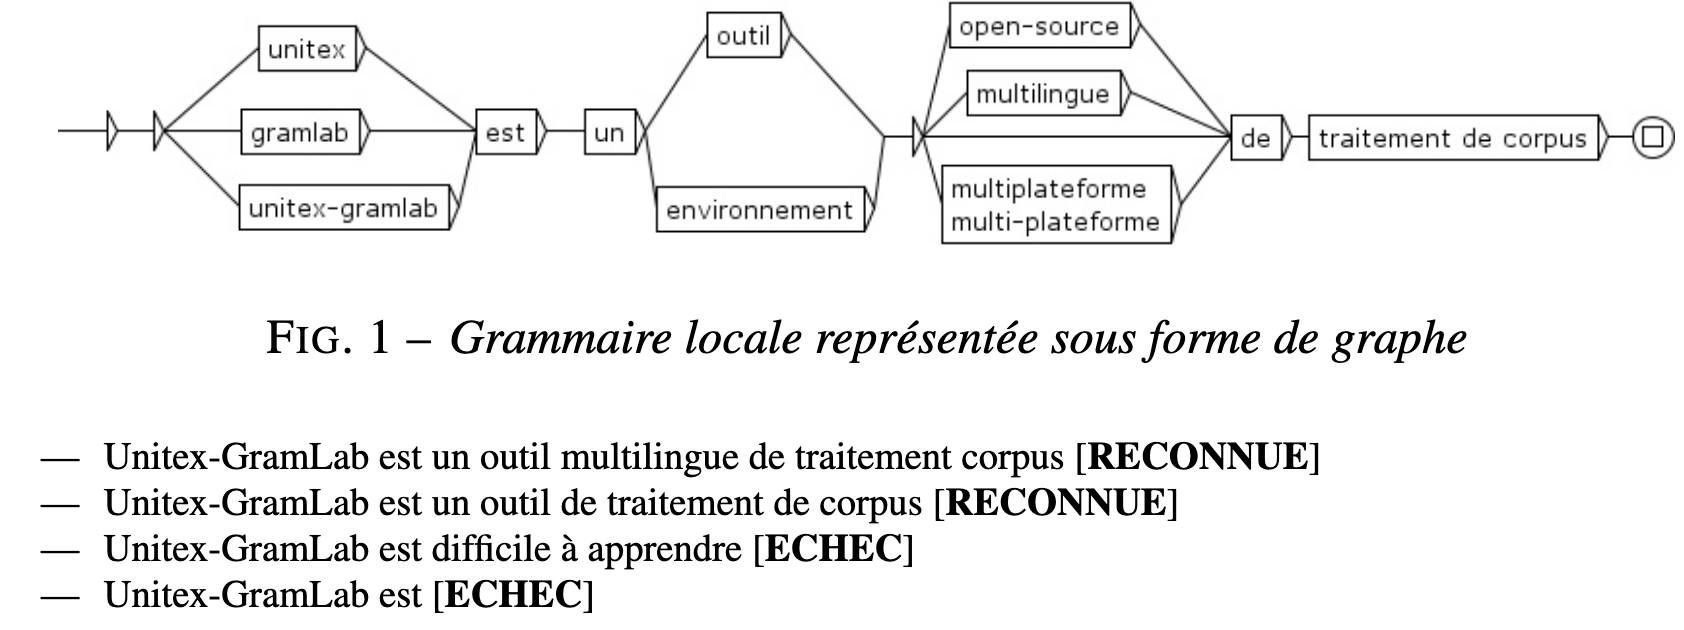
\includegraphics[width=1\linewidth]{img/grammaires_locales.png}
		\caption{\citep{kyriacopoulou2018unitex}.}
		\label{fig:ling_out_TAL}
	\end{figure}
\end{frame}

\begin{frame}{Transducteurs à états finis}
	
	{\small angl. \textit{\textbf{F}inite \textbf{S}tate \textbf{T}ransducer}}
	
	Machine abstraite fonctionnant sur le même
	principe que les \textsc{AFD}
	
	\begin{itemize}
		\item possibilité d'émettre un message à chaque transition
		\item capable de \textbf{reconnaissance} d'un
		langage formel, et de \textbf{production} d’une
		chaîne en sortie
		\item chaîne entrée $\rightarrow$ [transducteur] $\rightarrow$ chaîne sortie
	\end{itemize}

	
\end{frame}

\begin{frame}{Fonctionnement d'un transducteur : exemple de flexion}
		\begin{itemize}
					\item lecture de la chaîne d’entrée comme un
			automate à états finis
			\item à chaque transition, si un message est
			associé, il est émis
			\item aucun message ne sera émis
			si la chaîne n’est pas reconnue
		\item entrée : chaîne correspondant à un nom au
		singulier
		\item sortie : pluriel du nom fourni en entrée
		\begin{itemize}
			\item chat $\rightarrow$ chat\textbf{s} (exemple trivial)
			\item chev\textbf{al} $\rightarrow$ chev\textbf{aux} (exemple moins trivial)
		\end{itemize}
	\end{itemize}
	\resizebox{0.8\textwidth}{!}{
		\begin{tikzpicture}[shorten >=1pt, node distance=2.5cm, on grid, auto]
		% Define the states
		\node[state, initial] (q0) {0};
		\node[state, right=of q0] (q1) {1};
		\node[state, right=of q1] (q2) {2};
		\node[state, above right=of q2] (q3) {3};
		\node[state, accepting, right=of q3] (q4) {4};
		\node[state, below right=of q2] (q5) {5};
		\node[state, right=of q5] (q6) {6};
		\node[state, accepting, right=of q6] (q7) {7};
		
		% Transitions
		\path[->]
		(q0) edge node[above] {c : c} (q1)
		(q1) edge node[above] {h : h} (q2)
		(q2) edge node[above left] {a : a} (q3)
		(q2) edge node[below left] {i : i} (q5)
		(q3) edge node[above] {t : ts} (q4)
		(q5) edge node[above] {e : e} (q6)
		(q6) edge node[above] {n : ns} (q7);
	\end{tikzpicture}
}
\end{frame}

\begin{frame}{Utilisations de transducteurs en TAL}
	\bolder{Phonétisation} (\textit{text to speech})
	\begin{itemize}
		\item entrée : chaîne de caractères orthographique
		\item sortie : chaîne de symbole phonétiques
	\end{itemize}
	\bolder{Segmentation}
	\begin{itemize}
		\item entrée : chaîne de caractères (texte ou phrase)
		\item sortie : séquence de phrases, de mots ou de
		morphèmes
	\end{itemize}
	\bolder{Analyse d'unités lexicales}
	\begin{itemize}
		\item entrée : mot
		\item sortie : informations diverses sur le mot 
		\begin{itemize}
			\item
			informations morphosyntaxiques, équivalents multilingues etc.
		\end{itemize}
	\end{itemize}
\end{frame}

\begin{frame}{Phonétisation}
Comment se prononce la lettre \og{}p\fg{} ?
	
		
		\begin{tikzpicture}[shorten >=1pt, node distance=3.5cm, on grid, auto]
			% Define states
			\node[state, initial] (q0) {0};
			\node[state, right=of q0] (q1) {1};
			\node[state, right=of q1] (q2) {2};
			
			% Transitions
			\path[->]
			(q0) edge node[above] {p:-} (q1)
			(q1) edge[bend left] node[above] {h: 'F'} (q2)
			(q1) edge node[above] {p: 'P'} (q2)
			(q1) edge[bend right] node[below] {l: 'PL'} (q2);
		\end{tikzpicture}
		

	
\end{frame}

\begin{frame}{Segmentation d'un texte}
Le point est-il une fin de phrase ou un élément d'un sigle ?


		\resizebox{0.8\textwidth}{!}{
	\begin{tikzpicture}[shorten >=1pt, node distance=4.5cm, on grid, auto]
		% Define states
		\node[state, initial] (q0) {0};
		\node[state, right=of q0] (q1) {1};
		\node[state, right=of q1] (q2) {2};
		\node[state, below left=of q1] (q3) {3};
		\node[state, below right=of q3] (q4) {4};
		
		% Transitions
		\path[->]
		(q0) edge node[above right] {A-Z} (q3)
		(q0) edge node[above] {a-z} (q1)
		(q1) edge[loop above] node {a-z} ()
		(q1) edge node[above] {\scriptsize (point) : [FIN DE PHRASE]} (q2)
%		(q3) edge node[above left] {(point)} (q4)
		(q3) edge[right] node[below left] {(point)} (q4)
		(q4) edge[bend right] node[right] {A-Z} (q3)
		(q3) edge[bend right=15] node[below right] {a-z} (q1);
		
	\end{tikzpicture}
}
\end{frame}

\begin{frame}{Analyse morphosyntaxique}
		
		Catégories des mots de la famille \og{}francis$\dots$\fg{}

\centering
\resizebox{1\textwidth}{!}{ % Adjust the size dynamically
	\begin{tikzpicture}[shorten >=1pt, node distance=5cm, on grid, auto]
		% Define states
		\node[state, initial] (q0) {0};
		\node[state, right=of q0] (q1) {1};
		\node[state, accepting, above right=of q1] (q5) {5};
		\node[state, right=of q1, accepting] (q6) {6};
		\node[state, below right=of q1] (q2) {2};
		\node[state, accepting, right=of q2] (q4) {4};
		\node[state, accepting, above right=of q2] (q3) {3};
		
		% Transitions
		\path[->]
		(q0) edge node[above] {francis} (q1)
		(q1) edge node[above] {\begin{tabular}{c} ation \\ N \end{tabular}} (q6)
%		(q1) edge node[below] {\begin{tabular}{c} ab \end{tabular}} (q6)
		(q1) edge[bend left] node[left] {\begin{tabular}{c} er \\ V \end{tabular}} (q5)
		(q1) edge[bend right] node[right] {ab} (q2)
		(q2) edge node[above] {\begin{tabular}{c} le \\ ADJ \end{tabular}} (q3)
		(q2) edge node[below] {\begin{tabular}{c} ilité \\ N \end{tabular}} (q4);
	\end{tikzpicture}
}
\end{frame}


\section{Unitex}
\begin{frame}{À propos d'Unitex}
	\begin{itemize}
		\item suite logicielle\footnote{\url{https://unitexgramlab.org/fr}} pour l'analyse des corpus 
		\item fondée sur des ressources linguistiques :
		\begin{itemize}
			\item dictionnaires électroniques
			\item grammaires locales
			\item tables lexico-syntaxiques (lexique-grammaire)
		\end{itemize}
		\item multiplateforme, multilingue
		\item documentation \citep{paumier2021unitex}\footnote{\url{https://unitexgramlab.org/releases/3.1/man/Unitex-GramLab-3.1-usermanual-fr.pdf}}
		\item tutoriels 
		\begin{itemize}
			\item en français (univ. de Tours)\footnote{\url{https://tln.lifat.univ-tours.fr/version-francaise/ressources/tutoriels-unitex}}
			\item en anglais \citep{krstev2022}
		\end{itemize}
	\end{itemize}
	
\end{frame}

\begin{frame}{Applications}
	\begin{itemize}
		\item recherche de motifs complexes dans des textes
		\item concordance (visualisation des résultats en contexte)
		\item annotation
		\item analyse
		\end{itemize}
	
		$\rightarrow$ par la création de grammaires locales ou de transducteurs \\
		$\rightarrow$ via une interface graphique
\end{frame}

\begin{frame}{Prétraitements du corpus}
		\begin{figure}[h] % Use [H] to force the figure to stay in place
		\centering
		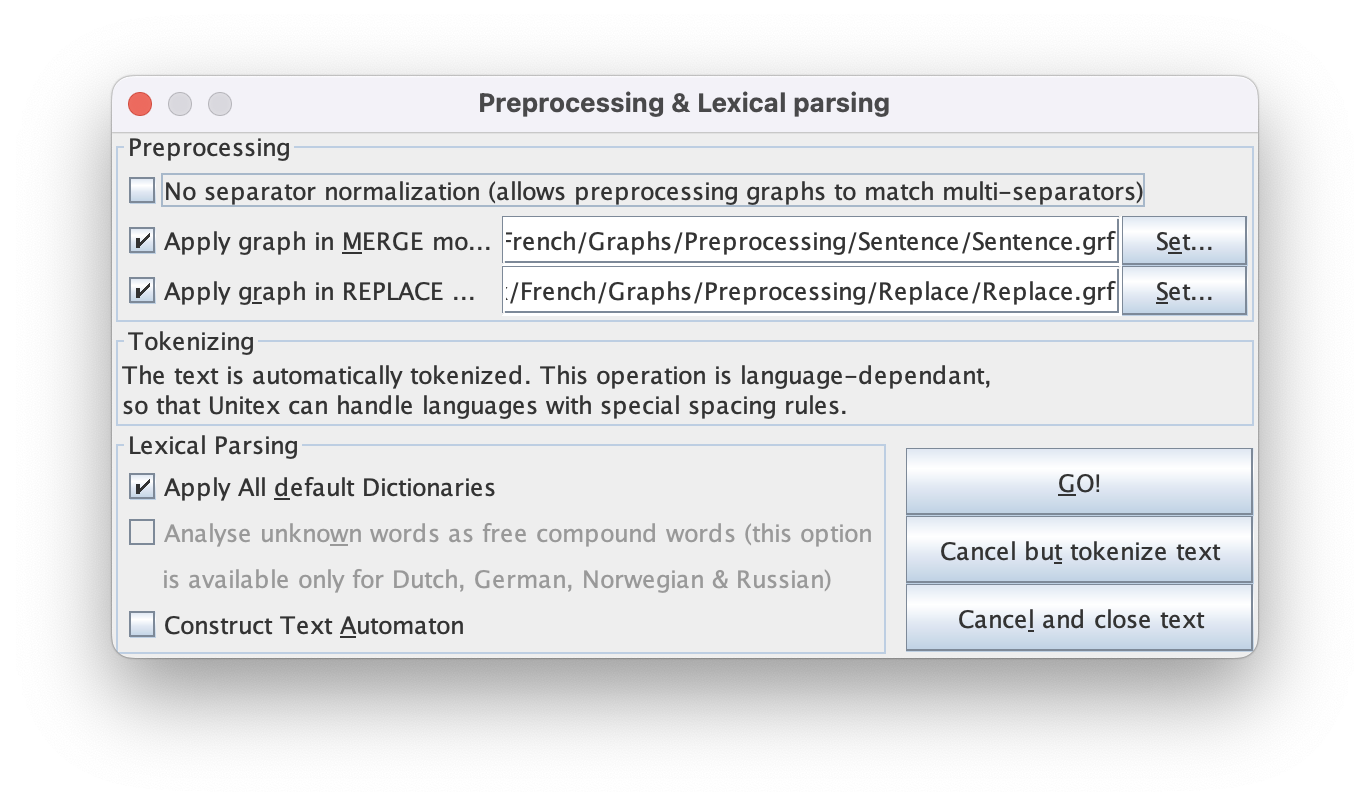
\includegraphics[width=0.7\linewidth]{img/pretraitement.png}
		\caption{Prétraitement du corpus \textit{Tour du monde en 80 jours} de Jules Verne.}
		\label{fig:ling_out_TAL}
	\end{figure}
\end{frame}

\begin{frame}{Prétraitements du corpus}
	\begin{itemize}
		\item \Colorbox{mygray}{\lstinline|Apply graph in MERGE mode|} 
		\begin{itemize}
			\item découpage du texte en phrases (délimiteur \texttt{S})
		\end{itemize} 
		\item \Colorbox{mygray}{\lstinline|Apply graph in REPLACE mode|} 
		\begin{itemize}
			\item normalisations de formes non ambiguës (\textit{puisqu'} $\rightarrow$ \textit{puisque})
		\end{itemize}
		\item découpage en unités lexicales : tokenisation
		\item \Colorbox{mygray}{\lstinline|Apply All default Dictionaries|} 
		\begin{itemize}
			\item  appliquer au texte des dictionnaires au format \textsc{DELA}\footnote{Dictionnaires Électroniques du \textsc{LADL}}
		\end{itemize}
		\item construction de l'automate du texte
	\end{itemize}
\end{frame}

\begin{frame}{Corpus prétraité}
			\begin{figure}[h] % Use [H] to force the figure to stay in place
		\centering
		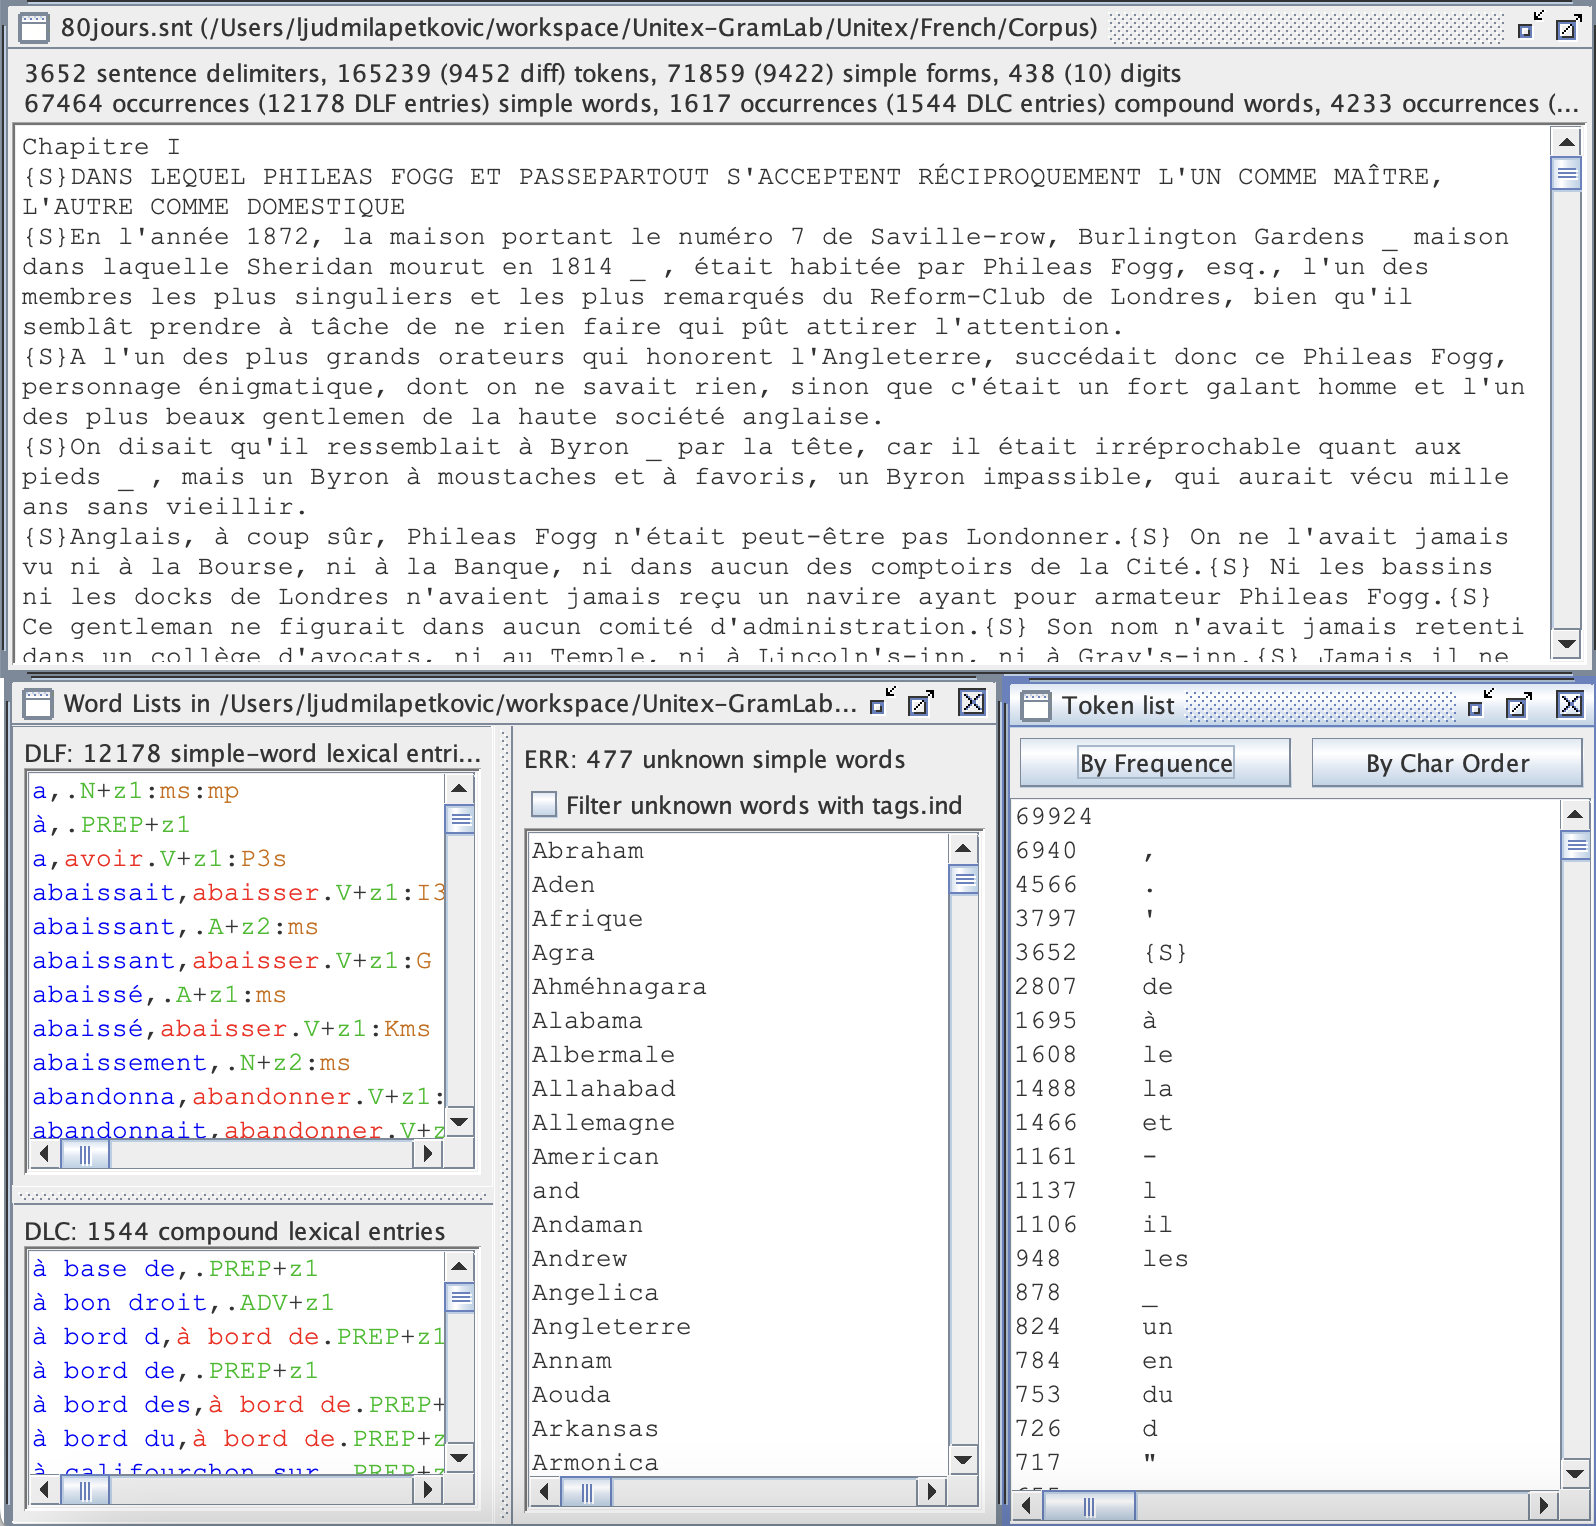
\includegraphics[width=0.65\linewidth]{img/corpus_pretraite.png}
		\caption{Corpus, liste de mots et de tokens.}
		\label{fig:ling_out_TAL}
	\end{figure}
\end{frame}

\begin{frame}{Corpus prétraité : statistiques}
	\begin{itemize}
		\item \textsc{3 652} délimiteurs de phrases
		\item \textsc{165 239} tokens
		\item \textsc{9 452} types
		\item \textsc{9 422} formes simples (\textsc{DLS}\footnote{\textsc{DELA} de formes Simples}, lemmes)
		\item \textsc{10} chiffres (types)
		\item \textsc{12 178} mots simples (\textsc{DLF}\footnote{\textsc{DELA} de formes Fléchies}, entrées)
		\item \textsc{1 544} mots composés (\textsc{DLC}\footnote{\textsc{DELA} de formes Composées}, entrées)
		\item \textsc{477} mots inconnus (\textsc{ERR}, entrées)
	\end{itemize}
\end{frame}

\begin{frame}{Dictionnaires Unitex}
	\begin{enumerate}
		\item dictionnaires de formes simples (\textsc{DELAS})
		\item dictionnaires de formes fléchies (\textsc{DELAF})
	\end{enumerate}
	qui comprennent des formes simples ou composées (\textsc{DELAC})
	\medskip
	
	\textsc{DELAS} :
	\texttt{cheval,N4,Anl}
	
	\textsc{DELAF} :\\
	\texttt{mercantiles,mercantile.A+z1:mp:fp}
	\texttt{grand=mères,grand=mère.N:fp}
\end{frame}

\begin{frame}{Contenu d'un dictionnaire Unitex}
	Ensemble d'entrées lexicales :
	\begin{itemize}
		\item forme de base (canonique, lemme) : \texttt{Descartes}
		\item catégorie grammaticale : nom (\texttt{N})
		\item informations flexionnelles (genre, nombre) : \texttt{ms}
		\item forme fléchie : \texttt{René Descartes}
		\item traits syntactico-sémantiques : \texttt{Hum+NPropre}
	\end{itemize}
	
	
	\begin{block}{Exemple}
		\justifying
		\texttt{Descartes,René Descartes.N+Hum+NPropre:ms}
	\end{block}
\end{frame}


\begin{frame}{Construction des dictionnaires}
	\begin{enumerate}
		\item dictionnaire de formes canoniques (ou formes de base)
		\item modules de flexion automatique (transducteurs)
		\item à chaque forme de base, on associe une classe flexionnelle \begin{itemize}
			\item un ensemble de règles
		\end{itemize}
	\end{enumerate}
	
	\begin{center}
		\textsc{DELAS} $\rightarrow$ Flexion automatique \textsc{DELAF}
	\end{center}
\end{frame}


\begin{frame}{Gestion du multilinguisme}
	Les traitements sont tous dépendants des langues :
	\begin{itemize}
		\item avantages : précision, adaptation aux spécificités
		\item inconvénients : lourdeur, maintenance compliquée
	\end{itemize}
	Alphabets : 
	\begin{itemize}
		\item un fichier qui définit les caractères d'une langue (\texttt{Alphabet.txt})
		\item un fichier indiquant les préférences pour le tri (\texttt{Alphabet\_sort.txt })
	\end{itemize}
\end{frame}

\begin{frame}{Alphabets}
		Ouvrir l'alphabet du français :
	\begin{itemize}
		\item que manque-t-il ? Comment est-ce géré ?
	\end{itemize}
	
	$\rightarrow$ p. ex. ligatures françaises : \ae{}, \AE{}, \oe{}, \OE{}
	
	Pour certaines langues comme le français, il arrive qu’à une lettre minuscule correspondent plusieurs majuscules.
	\begin{itemize}
		\item \texttt{é} $\rightarrow$ \texttt{E} ou \texttt{É}
		\item[] \texttt{Ee}, \texttt{Eé}, \texttt{Éé}, \texttt{Eè}, \texttt{Èè}, \texttt{Eë}, \texttt{Ëë}, \texttt{Eê}, \texttt{Êê}
	\end{itemize}
\end{frame}



\begin{frame}{Mots simples \textit{vs.} composés}
	\begin{block}{Mot simple}
		Une séquence de lettres délimitée par des séparateurs (espaces, ponctuation etc.) : \textit{pomme}
	\end{block}
	
		\begin{block}{Mot composé}
		Une séquence de mots simples dont le sens est non compositionnel : \textit{cordon bleu}, \textit{pomme de terre}, \textit{belle famille}, \textit{porte-manteau}, etc.
	\end{block}
\end{frame}

\begin{frame}{Exemples de recherches de motifs}
	\begin{itemize}
		\item un mot (\texttt{juger}) ou séquence de mots (\texttt{pomme de terre})
		\item toutes les formes fléchies associées à une forme de base (\texttt{<juger>} = \textit{juge}, \textit{juges}, \textit{jugeons}, etc.)
		\item formes appartenant à une catégorie grammaticale avec informations flexionnelles : \texttt{<N>}, \texttt{<N:ms>}, \texttt{<V:K>}
		\item motifs complexes : \texttt{<DET:ms><N:ms>}
		\item regex : \texttt{je+tu+il+elle+on+nous+vous+ils+elles}
		\item automates sous la forme de graphes
	\end{itemize}
\end{frame}
\begin{frame}{Recherches simples}
	\begin{enumerate}
		\item rechercher le motif \texttt{parler} en cliquant sur \texttt{Locate Pattern} dans le menu \texttt{Text}
		\begin{itemize}
			\item regarder le résultat avec le concordancier
			\item modifier les différentes options et observer les résultats
		\end{itemize}
		\item même question avec le motif \texttt{<parler>}
		\item même question avec le motif \texttt{<V:P3p>}
		\item à quoi correspondent les motifs précédents ?
	\end{enumerate}
\end{frame}

\begin{frame}{\texttt{Locate Pattern} et concordancier}
		   \begin{figure}[ht]
		\begin{minipage}[b]{0.45\linewidth}
			\centering
			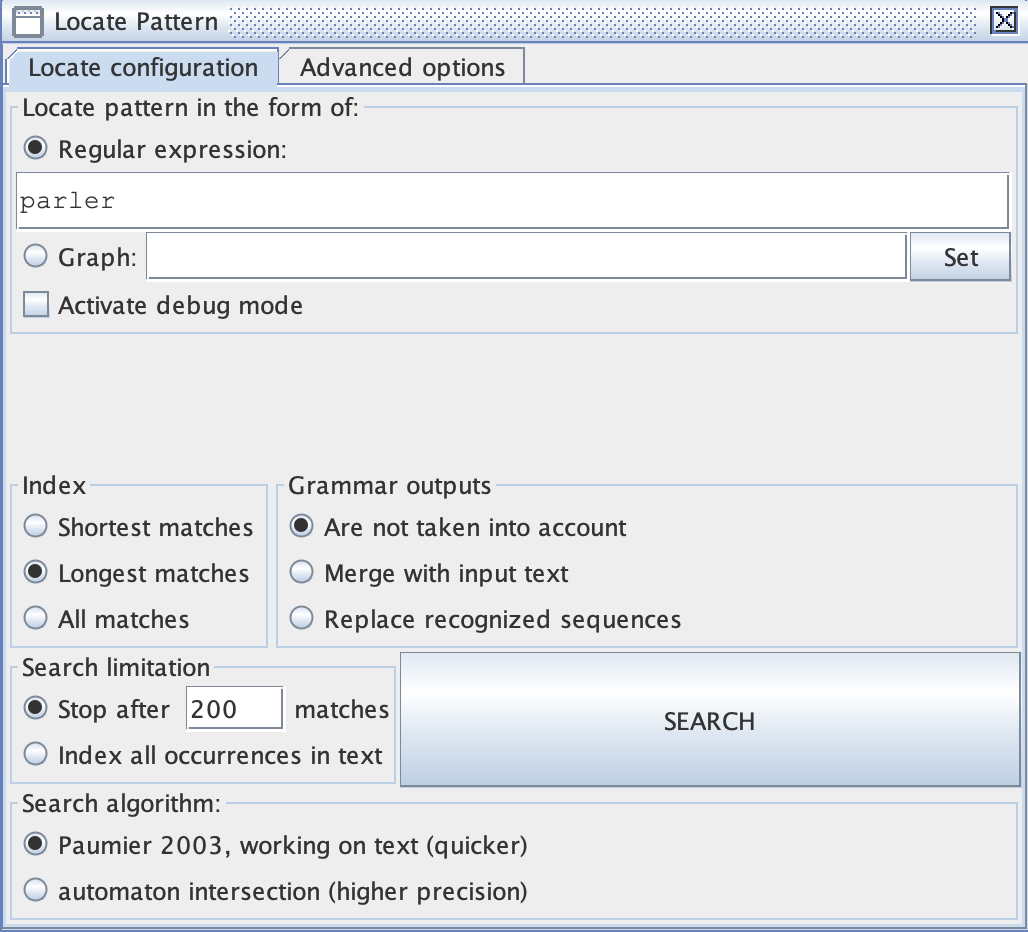
\includegraphics[width=\textwidth]{img/locate_pattern.png}
			\caption{\texttt{Locate Pattern}.}
			\label{fig:a}
		\end{minipage}
		\hspace{0.5cm}
		\begin{minipage}[b]{0.45\linewidth}
			\centering
			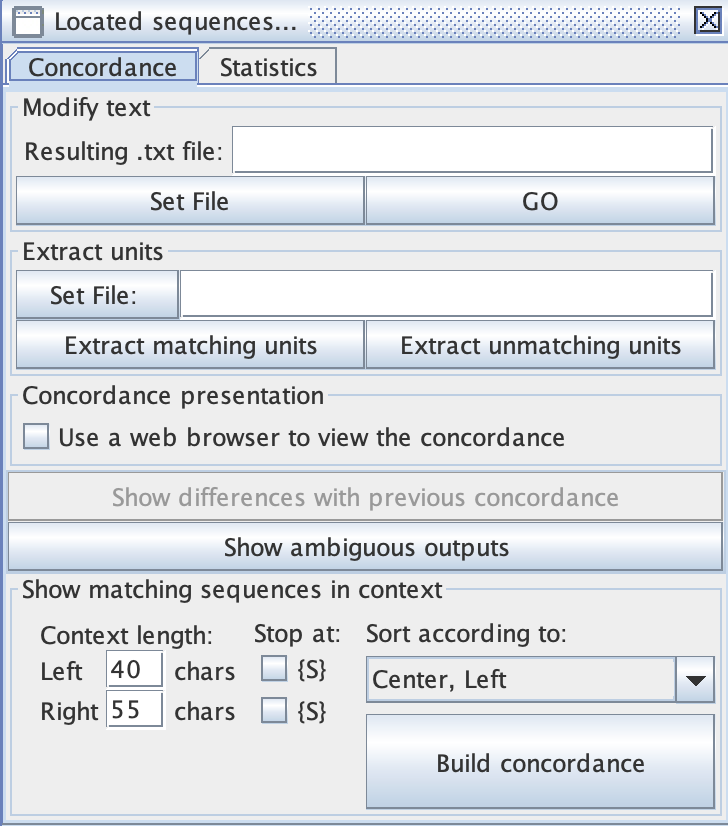
\includegraphics[width=\textwidth]{img/concordancier.png}
			\caption{Lancer le concordancier.}
			\label{fig:b}
		\end{minipage}
	\end{figure}
	
\end{frame}

\begin{frame}{Expression régulières ou rationnelles (regex)}
	Une regex peut être :
	\begin{itemize}
		\item une \textcolor{deepblue}{unité lexicale} (\texttt{livre}) ou un masque lexical (\texttt{<manger.V>})
		\item une \textcolor{deepblue}{position} particulière du texte : le début (\texttt{\^}) ou la fin \texttt{\$}
		\item la \textcolor{deepblue}{concaténation} de deux regex (\texttt{je mange})
		\item l'\textcolor{deepblue}{union} de deux regex (\texttt{Pierre+Paul})
		\item l'\textcolor{deepblue}{étoile de Kleene} d'une regex (\texttt{très*})
	\end{itemize}
\end{frame}

\begin{frame}{Concordancier}
			\begin{figure}[h] % Use [H] to force the figure to stay in place
		\centering
		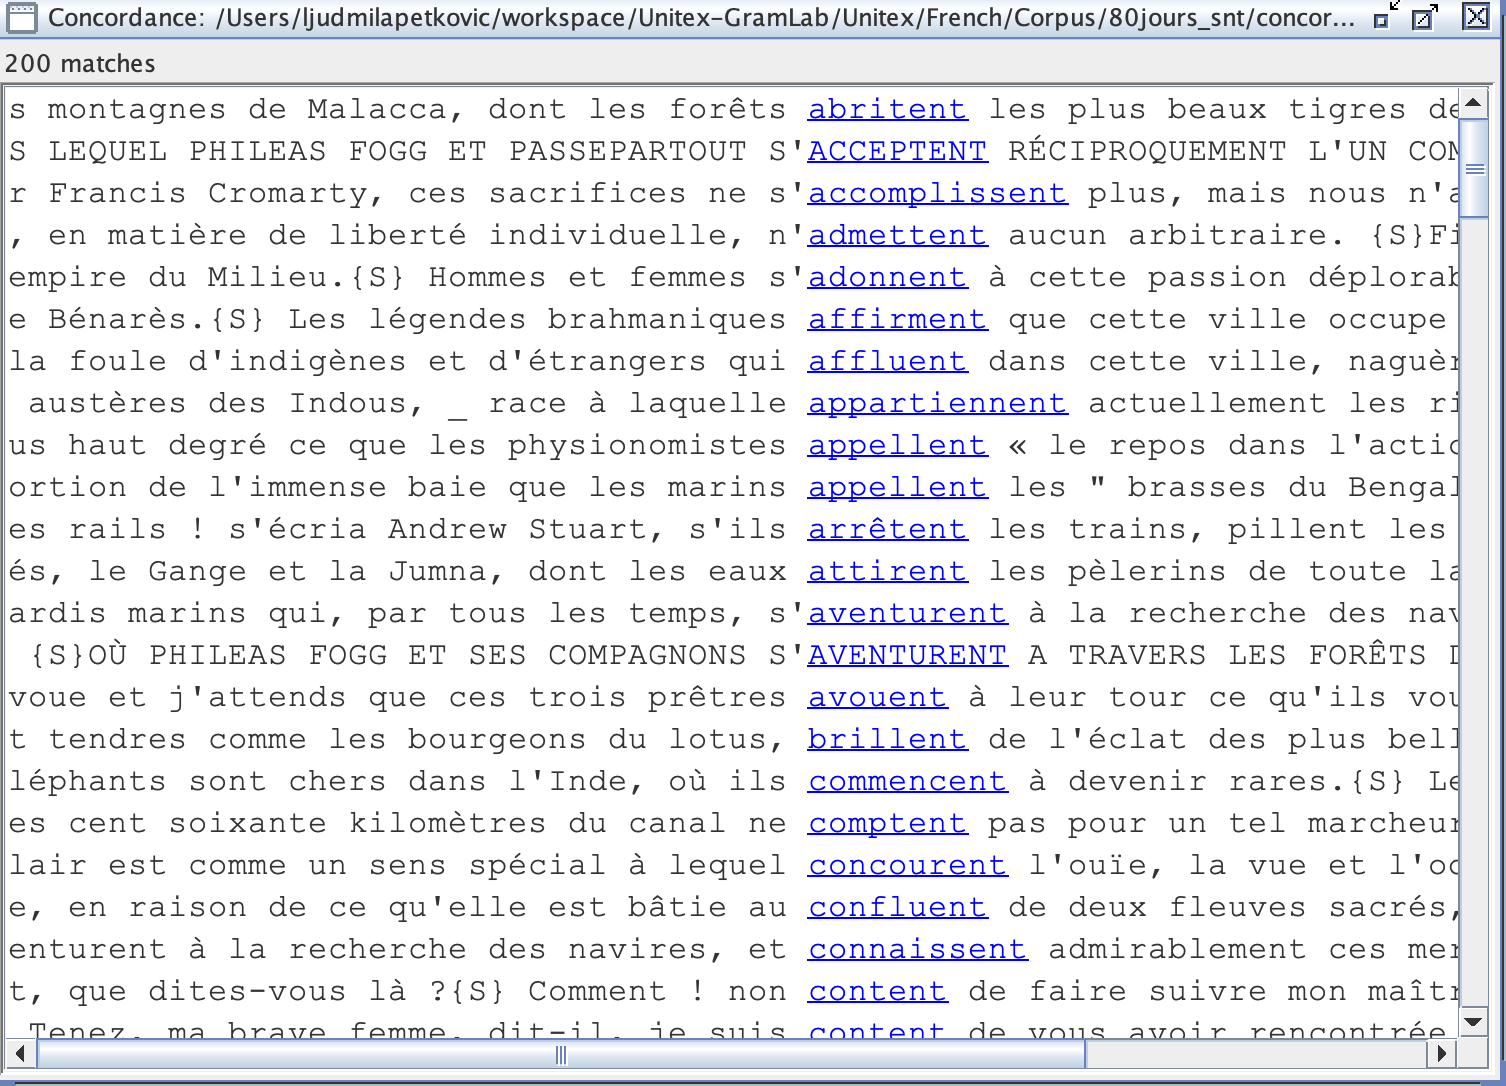
\includegraphics[width=0.8\linewidth]{img/concordance.png}
		\caption{Concordance sur le motif \texttt{V:P3p} -- verbes de la 3\textsuperscript{e} personne du pluriel.}
		\label{fig:ling_out_TAL}
	\end{figure}
\end{frame}

\begin{frame}{Statistiques de collocations}
	\begin{figure}[h] % Use [H] to force the figure to stay in place
		\centering
		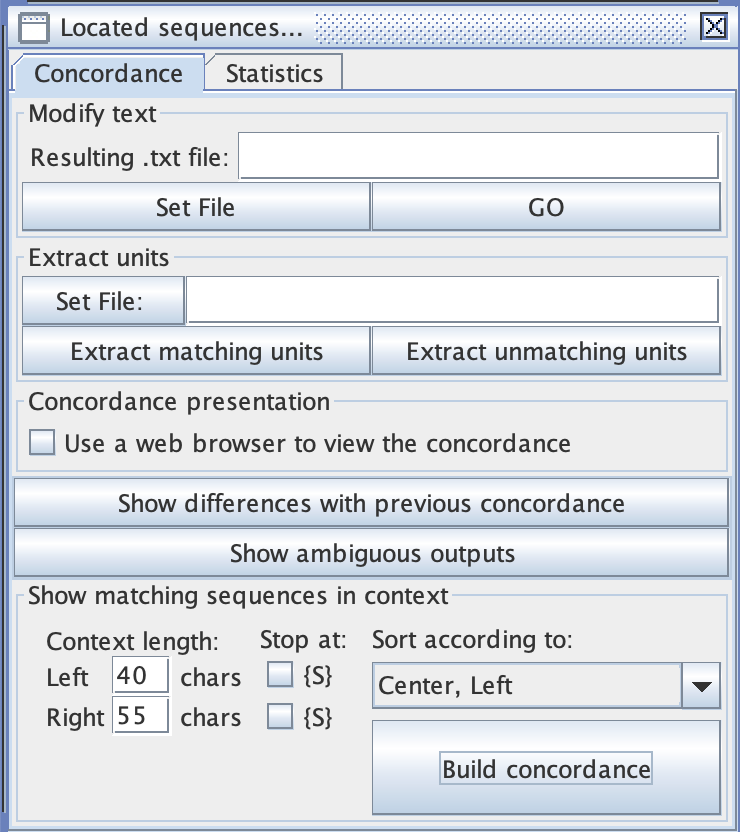
\includegraphics[width=0.6\linewidth]{img/collocations.png}
		\caption{Statistiques sur les séquences préalablement indexées.}
		\label{fig:ling_out_TAL}
	\end{figure}
\end{frame}

\begin{frame}{Collocations du motif \texttt{V:P3p}}
		\begin{figure}[h] % Use [H] to force the figure to stay in place
		\centering
		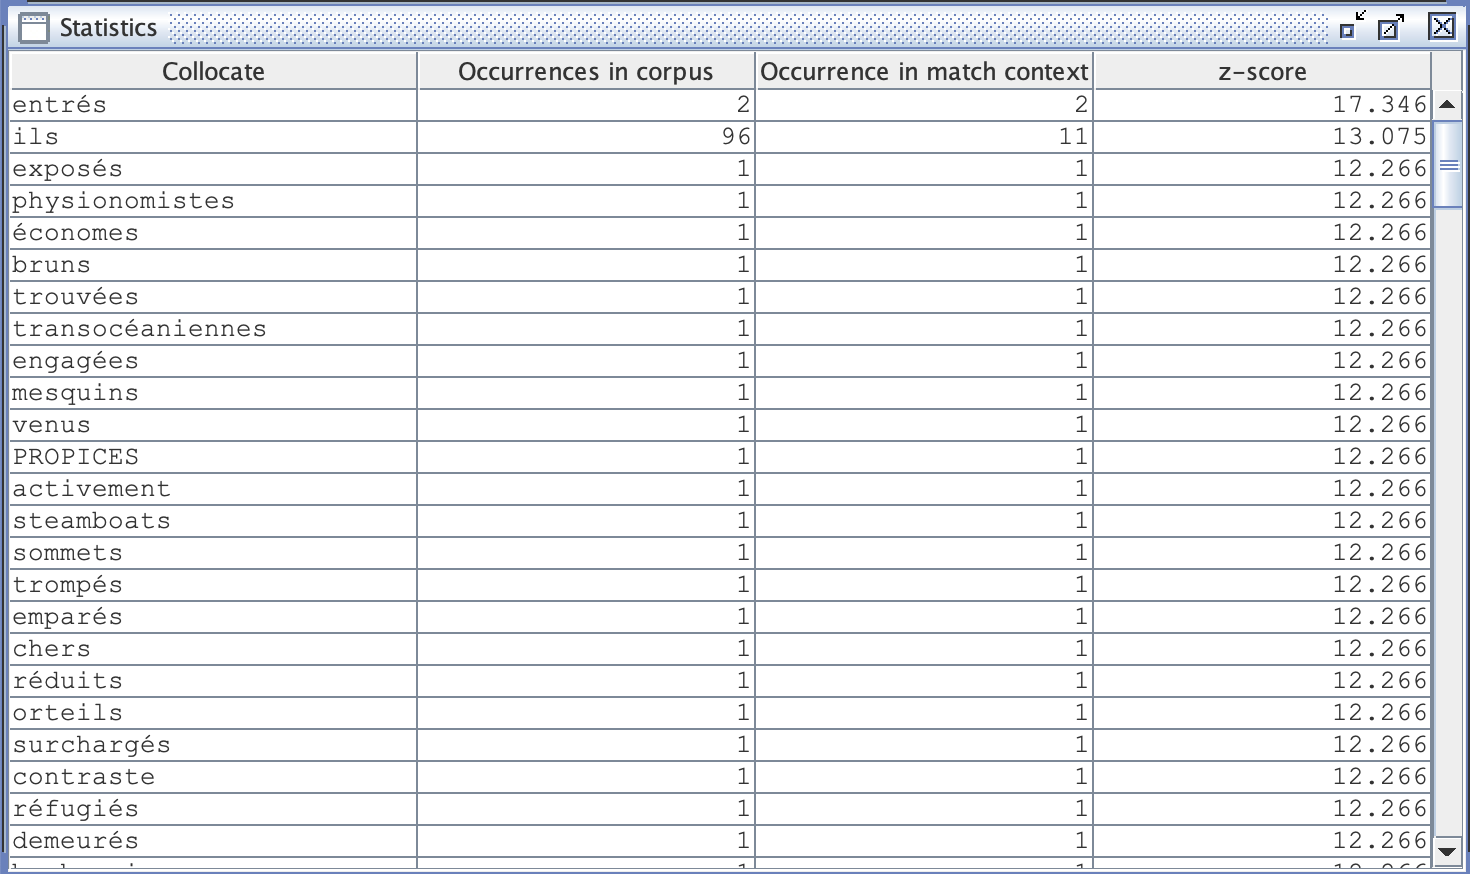
\includegraphics[width=0.8\linewidth]{img/resultats_collocations.png}
		\caption{Collocats, occurrences dans le corpus / contexte de cooccurrence, score \textit{z}.}
		\label{fig:ling_out_TAL}
	\end{figure}
\end{frame}


\begin{frame}{Opérateurs}
	\begin{itemize}
\item 	Concaténation
	\begin{itemize}
		\item point : \texttt{<DET>.<N>} : reconnaît un déterminant suivi par un nom
		\item espace : \texttt{le <A> chat} : reconnaît l'unité lexicale \textit{le}, suivie d'un adjectif et de l'unité lexicale \textit{chat}
		\item parenthèses : servent de délimiteurs 
	\end{itemize}
	
\item 	Union : 
	\begin{itemize}
		\item \texttt{+} : \texttt{chat+chien <v>} : reconnaît l'unité lexicale \textit{chat} ou \textit{chien}, suivie par un verbe
		\item epsilon : \texttt{le (petit+<E>) chat} : reconnaît les séquences \textit{le chat} et \textit{le petit chat}
	\end{itemize}
	
\item 	Étoile de Kleene \texttt{*} : reconnaît zéro, 1+ occur. d'une regex
	\begin{itemize}
		\item \texttt{il fait très* froid} : reconnaît \textit{il fait froid}, \textit{il fait très froid}, \textit{il fait très très froid} etc.
		\item prioritaire sur les autres opérateurs
		\item parenthèses pour appliquer l'étoile à une regex complexe
	\end{itemize}
	\end{itemize}
\end{frame}

\begin{frame}{Codes grammaticaux usuels}
			\begin{figure}[h] % Use [H] to force the figure to stay in place
		\centering
		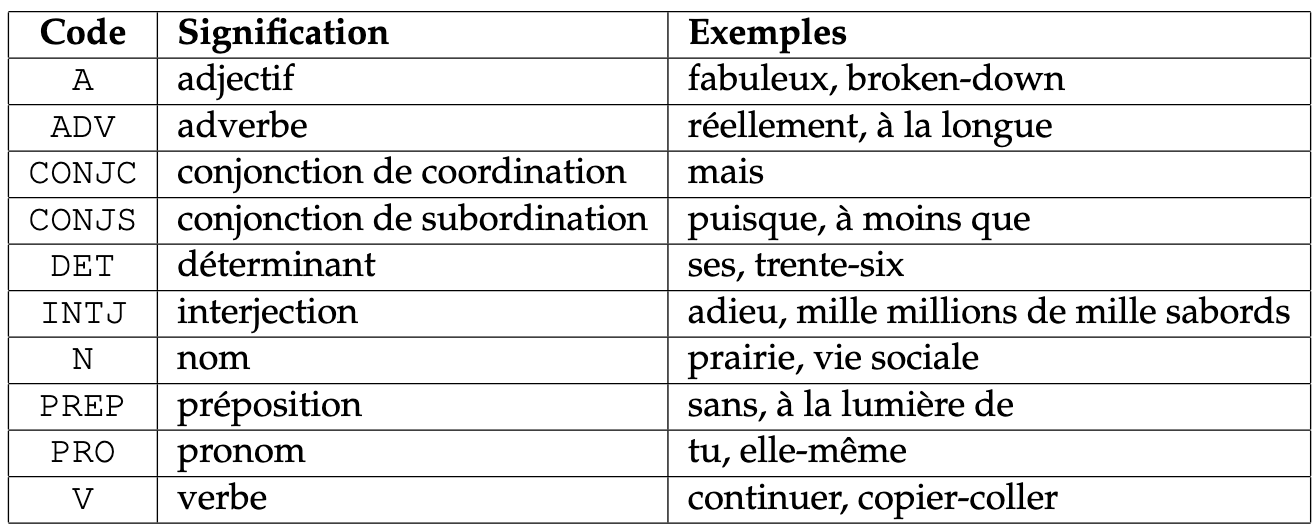
\includegraphics[width=1\linewidth]{img/codes_grammaticaux.png}
		\caption{Exemples de codes grammaticaux usuels.}
		\label{fig:ling_out_TAL}
	\end{figure}
\end{frame}

\begin{frame}{Codes sémantiques usuels}
	\begin{figure}[h] % Use [H] to force the figure to stay in place
		\centering
		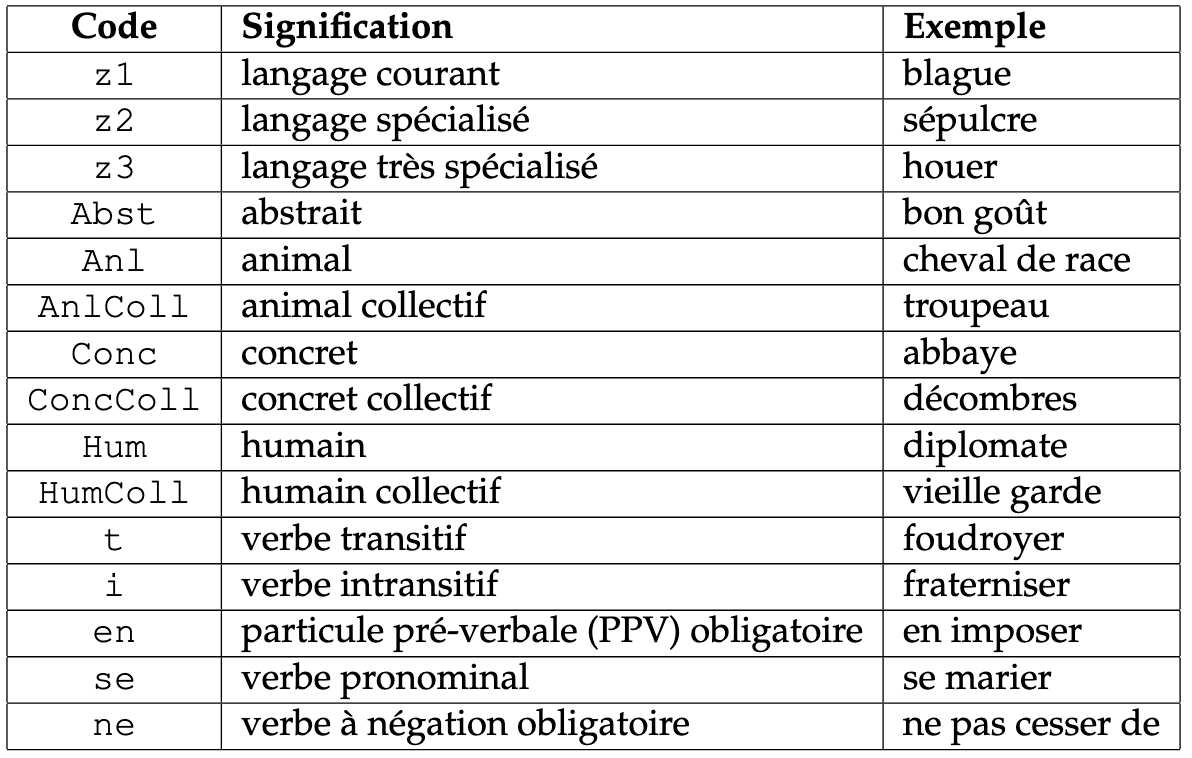
\includegraphics[width=1\linewidth]{img/codes_semantiques.png}
		\caption{Exemples de codes sémantiques usuels.}
		\label{fig:ling_out_TAL}
	\end{figure}
\end{frame}

\begin{frame}{Codes flexionnels usuels}
	\begin{figure}[h] % Use [H] to force the figure to stay in place
		\centering
		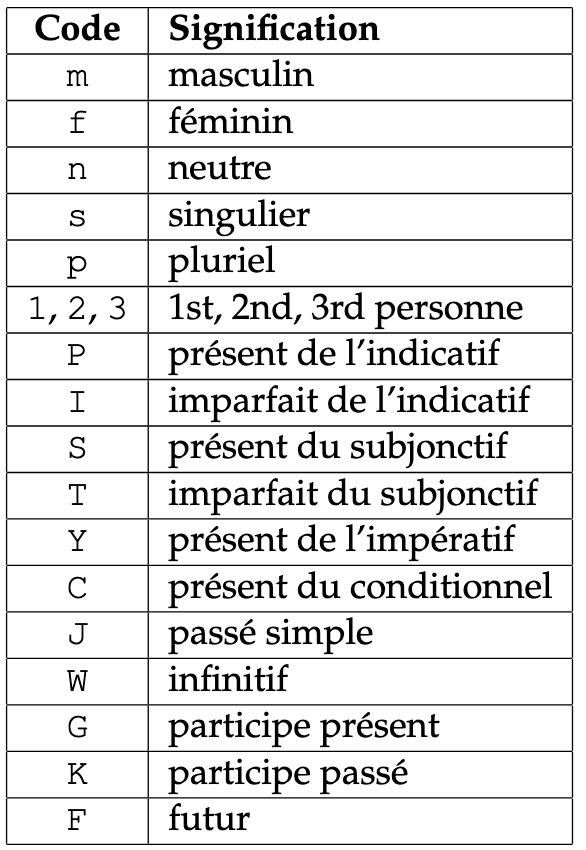
\includegraphics[width=.43\linewidth]{img/codes_flexionnels.png}
		\caption{Exemples de codes flexionnels usuels.}
		\label{fig:ling_out_TAL}
	\end{figure}
\end{frame}

\begin{frame}{Méta-motifs Unitex}
	\begin{itemize}
		\item \texttt{<E>} : mot vide, ou epsilon. Reconnaît la séquence vide
		\item \texttt{<TOKEN>} : n'importe quelle unité lexicale sauf l'espace
		\item \texttt{<MOT>} : n'importe quelle unité lexicale formée de lettres
		\item \texttt{<MIN>} : [$\dots$] de lettres minuscules
		\item \texttt{<MAJ>} : [$\dots$] de lettres majuscules
		\item \texttt{<PRE>} : [$\dots$] de lettres et commençant par une majuscule
		\item \texttt{<DIC>} : n'importe quel mot figurant dans les dictionnaires du texte
		\item \texttt{<SDIC>} : [$\dots$] mot simple [$\dots$]
		\item \texttt{<CDIC>} : [$\dots$] mot composé [$\dots$] 
		\item \texttt{<NB>} : n'importe quelle suite de chiffres contigus
	\end{itemize}
\end{frame}

\begin{frame}{Négation et interdiction}
	\begin{itemize}
		\item \texttt{!} (immédiatement après \texttt{<}) : négation d'un motif, possible sur :
		\begin{itemize}
			\item les métas \texttt{<MOT>}, \texttt{<MIN>}, \texttt{<MAJ>}, \texttt{<PRE>}, \texttt{<DIC>}
			\item les masques lexicaux ne comportant que des codes grammaticaux, sémantiques ou flexionnels (\texttt{<!V + z3 : P3})
		\end{itemize}
		\item \texttt{$\sim$} : exclut des codes (\texttt{<A$\sim$z3} reconnaît toutes les entrées qui ont le code \textit{A} sans le code \textit{z3})
		\item \texttt{\#} : interdit la présence de l'espace
	\end{itemize}
\end{frame}

\begin{frame}{Filtres morphologiques Unitex}
	\bolder{Format}
	
	motif $<<$motif morphologique$>>$\\
	sous la forme de regex au format \textsc{POSIX}\footnote{https://fr.wikipedia.org/wiki/Expression\_r\%C3\%A9guli\%C3\%A8re\#Expressions\_rationnelles\_.C3.A9tendues\_POSIX}
	
	Par défaut, un filtre morphologique tout seul s’applique au méta
	\texttt{<TOKEN>}, c’est-à-dire à n’importe quelle unité lexicale sauf l’espace.
\end{frame}

\begin{frame}{Filtres simples}
	\begin{itemize}
		\item \texttt{<<ss>>} : contient \textit{ss}
		\item \texttt{<<\^{}a>>} : commence par \textit{a}
		\item \texttt{<<ez\${}>>} : finit par \textit{ez}
		\item \texttt{<<a.*s>>} : contient \textit{a} suivi par un nombre de caractères quelconque, suivi par \textit{s}
		\item \texttt{<<ss|tt>>} : contient \textit{ss} ou \textit{tt}
		\item \texttt{<<[aeiouy]>>} : contient une voyelle non accentuée
		\item \texttt{<<[aeiouy]3,5>>} : contient une séquence de voyelles non accentuées, de longueur comprise entre 3 et 5
		\item \texttt{<<es?>>} : contient \textit{e} suivi par un \textit{s} facultatif
		\item \texttt{<<ss[\^{}e]?} : contient \textit{ss} suivi par un caractère qui n'est pas une voyelle \textit{e}
	\end{itemize}
\end{frame}

\begin{frame}{Filtres plus complexes}
	\begin{itemize}
		\item \texttt{<<[ai]ble\${}>>} : finit par \textit{able} ou \textit{ible}
		\item \texttt{<<\^{}[rst][aeiouy]{2,}\${}>>} : mot formé de 2 ou plus séquences commençant par un \textit{r}, \textit{s} ou \textit{t} suivi d'une voyelle non accentuée
	\end{itemize}
	
	Lorsqu'un filtre suit immédiatement un motif, il s'applique à ce qui est reconnu par le motif :
	\begin{itemize}
		\item \texttt{<V:K><<i\${}>>} : participe passé finissant par \textit{i}
		\item \texttt{<CDIC><<.*>>} : mot composé contenant deux espaces
		\item \texttt{<A:fs><<\^{}pro>>} : adjectif fém. sing. commençant par \textit{pro}
	\end{itemize}
\end{frame}

\begin{frame}{Créer un graphe simple}
	\begin{itemize}
		\item dans le menu \Colorbox{mygray}{\lstinline|FSGraph|}, sélectionner \Colorbox{mygray}{\lstinline|New...|}
		\item faire un \Colorbox{mygray}{\lstinline|Ctrl + clic|} entre l'état initial et l'état final
		\item pour supprimer un état, cliquer sur la tête de mort
		\item dans la barre de texte, à la place de \Colorbox{mygray}{\lstinline|<E>|}, taper : \Colorbox{mygray}{\lstinline|je+tu+il+elle+on+nous+vous+ils+elles|}
		\item taper \Colorbox{mygray}{\lstinline|Entrée|}
	\end{itemize}
\end{frame}

\begin{frame}{Graphe créé}
				\begin{figure}[h] % Use [H] to force the figure to stay in place
		\centering
		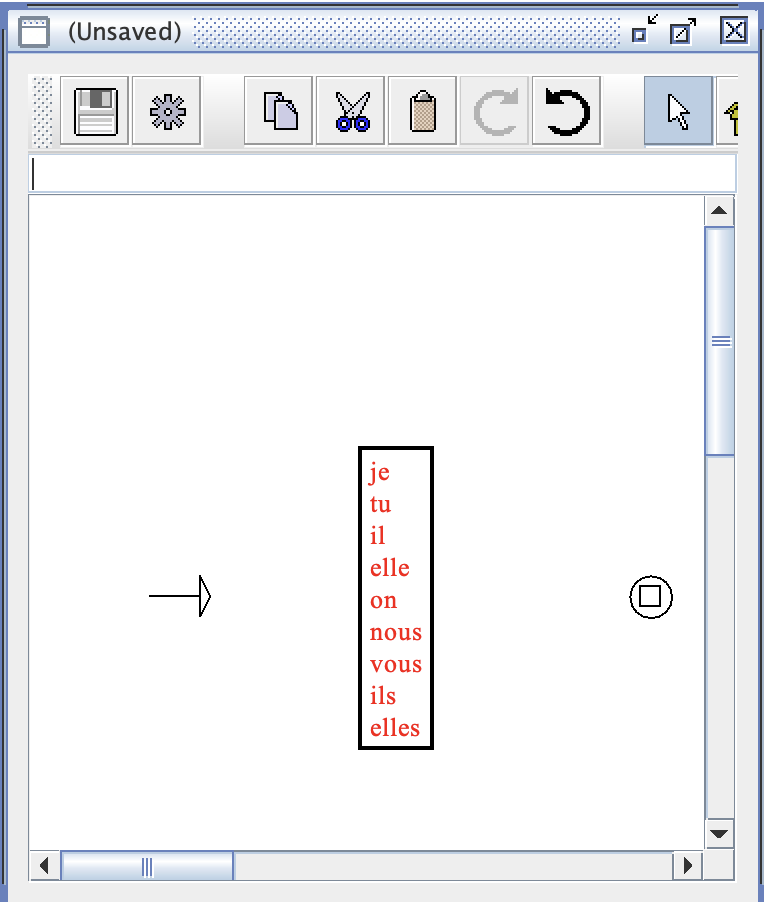
\includegraphics[width=.5\linewidth]{img/graphe.png}
		\caption{Mon premier graphe.}
		\label{fig:ling_out_TAL}
	\end{figure}
\end{frame}

\begin{frame}{Lier le graphe créé}
	\begin{itemize}
		\item cliquer sur la flèche de l'état initial, puis sur l'état \texttt{je+tu...} (une transition apparaît)
		\item pour supprimer une transition, refaire la même manipulation
	\end{itemize}
	\begin{figure}[h] % Use [H] to force the figure to stay in place
		\centering
		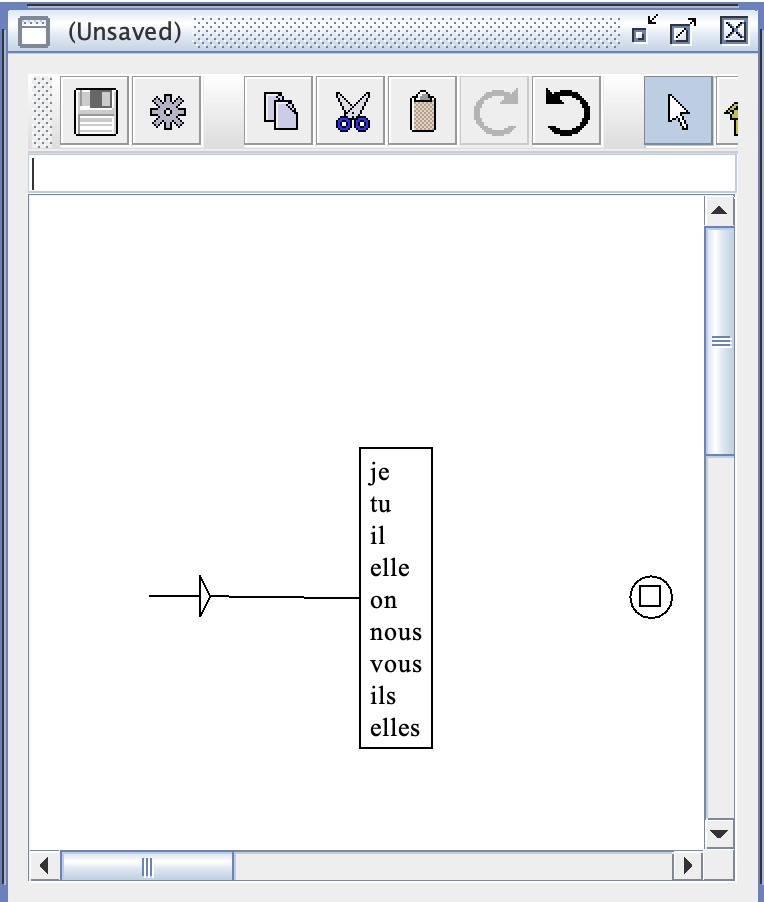
\includegraphics[width=.35\linewidth]{img/graphe_lie.png}
		\caption{Mon premier graphe lié de l'état initial.}
		\label{fig:ling_out_TAL}
	\end{figure}
\end{frame}

\begin{frame}{Compléter le graphe}
	\begin{itemize}
		\item cliquer sur l'état \texttt{je+tu...} puis sur l'état final (une transition apparaît)
			\begin{figure}[h] % Use [H] to force the figure to stay in place
			\centering
			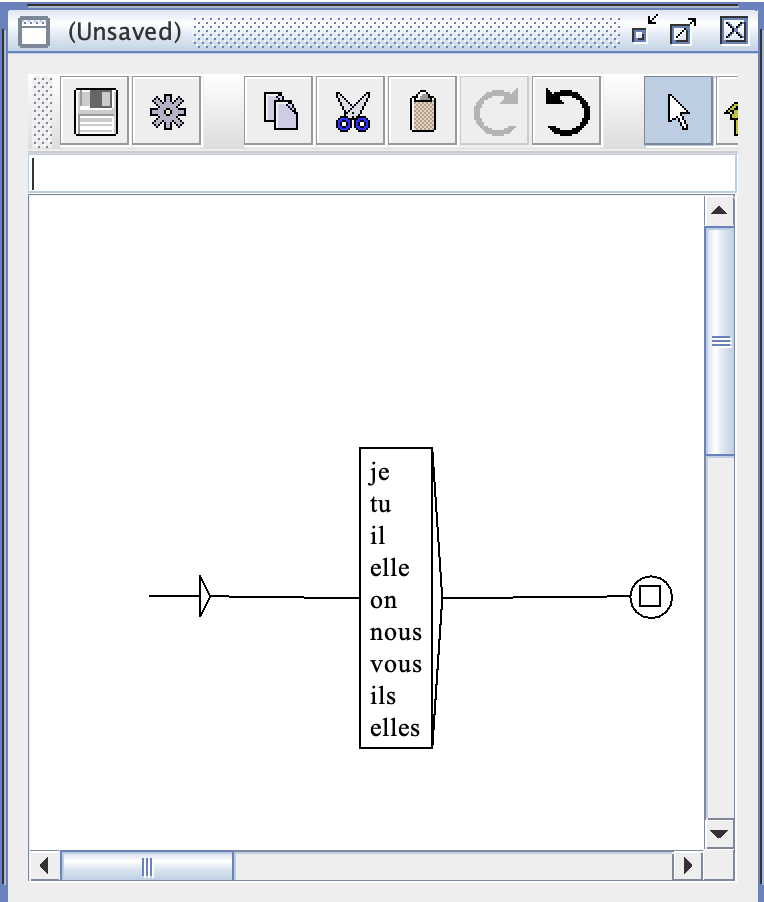
\includegraphics[width=.3\linewidth]{img/graphe_fini.png}
			\caption{Mon premier graphe lié de l'état initial.}
			\label{fig:ling_out_TAL}
		\end{figure}
		\item dans le menu \Colorbox{mygray}{\lstinline|FSGraph|}, sélectionner \Colorbox{mygray}{\lstinline|Save as...|} (pour enregistrer le graphe)
	\end{itemize}
\end{frame}

\begin{frame}{Appliquer le graphe à un texte}
	Pour appliquer le graphe au texte : 
	\begin{itemize}
		\item ouvrir un texte (p. ex. le \textit{Tour du monde en 80 jours})
		\item puis menu \Colorbox{mygray}{\lstinline|Text > Locate Pattern|}
		\item dans \Colorbox{mygray}{\lstinline|Graph|}, indiquer (\textit{set}) le chemin vers le graphe enregistré précédemment
	\end{itemize}
\end{frame}

\begin{frame}{Création d'une substitution}
	\textcolor{deepblue}{Remplacer une chaîne par une autre}
	\begin{itemize}
		\item créer un graphe à un état intermédiaire
		\item dans cet état, écrire \texttt{folie/démence}
		\item enregistrer ce graphe
	\end{itemize}
\end{frame}

\begin{frame}{Application d'un graphe avec substitution}
	\textcolor{deepblue}{Remplacer une chaîne par une autre}
	\begin{itemize}
		\item ouvrir un texte (p. ex. le \textit{Tour du monde en 80 jours})
		\item puis, menu \Colorbox{mygray}{\lstinline|Text > Locate Pattern > Graph|}
		\item dans \Colorbox{mygray}{\lstinline|Graph|}, indiquer \textit{set} le chemin vers le graphe enregistré
		\item selectionner \Colorbox{mygray}{\lstinline|Grammar Outputs > Replace recognized sentences|}
	\end{itemize}
				\begin{figure}[h] % Use [H] to force the figure to stay in place
		\centering
		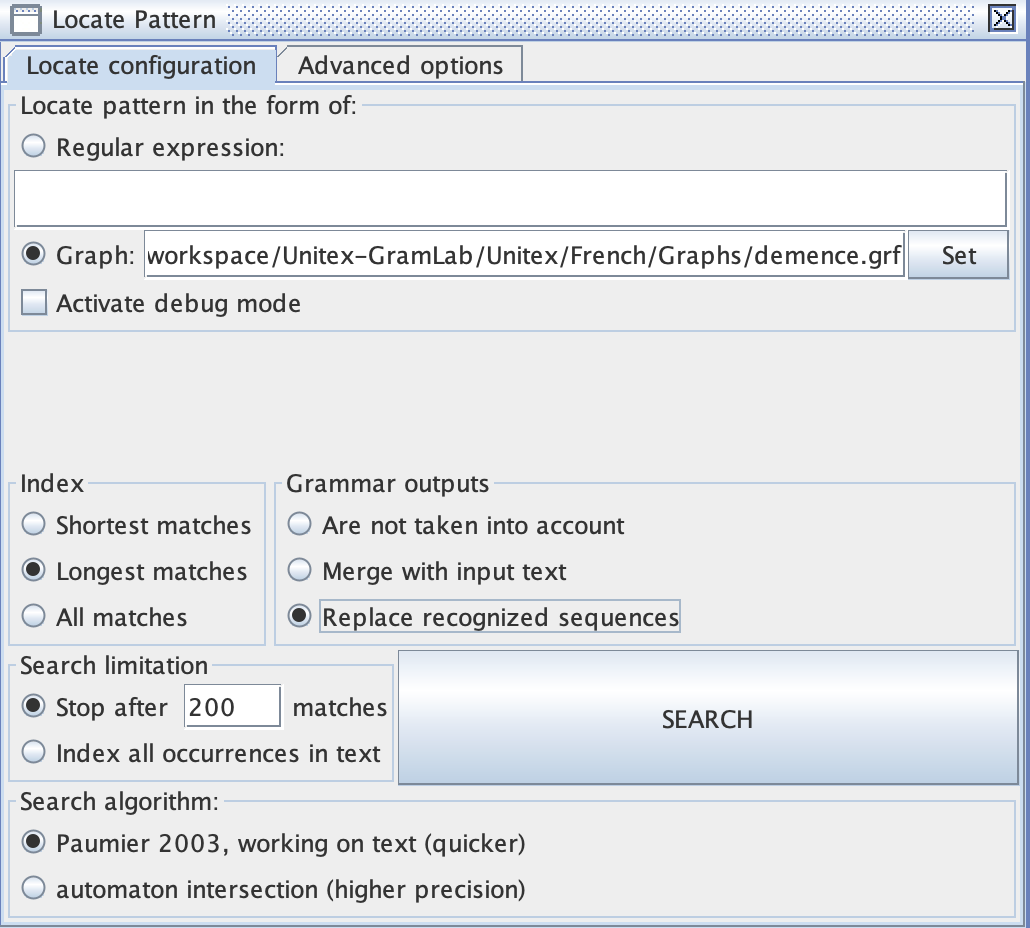
\includegraphics[width=.3\linewidth]{img/substitution.png}
		\caption{Mon premier graphe de substitution.}
		\label{fig:ling_out_TAL}
	\end{figure}
\end{frame}

\begin{frame}{Création d'une annotation}
	\textcolor{deepblue}{Annoter une chaîne de caractères}
	\begin{itemize}
		\item créer un graphe reconnaissant l'expression \textit{un des plus}
		\item écrire \texttt{un/<select>}
		\item ajouter après l'expression l'état contenant \texttt{<E>/</select>}
		\item enregistrer le graphe
	\end{itemize}
					\begin{figure}[h] % Use [H] to force the figure to stay in place
		\centering
		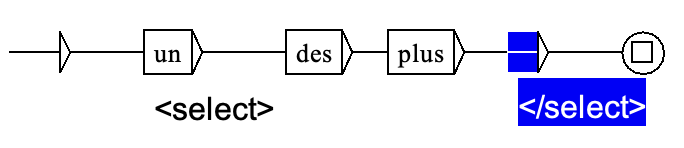
\includegraphics[width=.5\linewidth]{img/un_des_plus.png}
		\caption{Mon premier graphe d'annotation.}
		\label{fig:ling_out_TAL}
	\end{figure}
\end{frame}

\begin{frame}{Appliquer les annotations dans le texte}
\textcolor{deepblue}{Annoter le texte}
		\begin{itemize}
		\item ouvrir un texte (p. ex. le \textit{Tour du monde en 80 jours})
		\item puis, menu \Colorbox{mygray}{\lstinline|Text > Locate Pattern > Graph|}
		\item selectionner \Colorbox{mygray}{\lstinline|Grammar Outputs > Merge with input text|}
	\end{itemize}
			\begin{figure}[h] % Use [H] to force the figure to stay in place
		\centering
		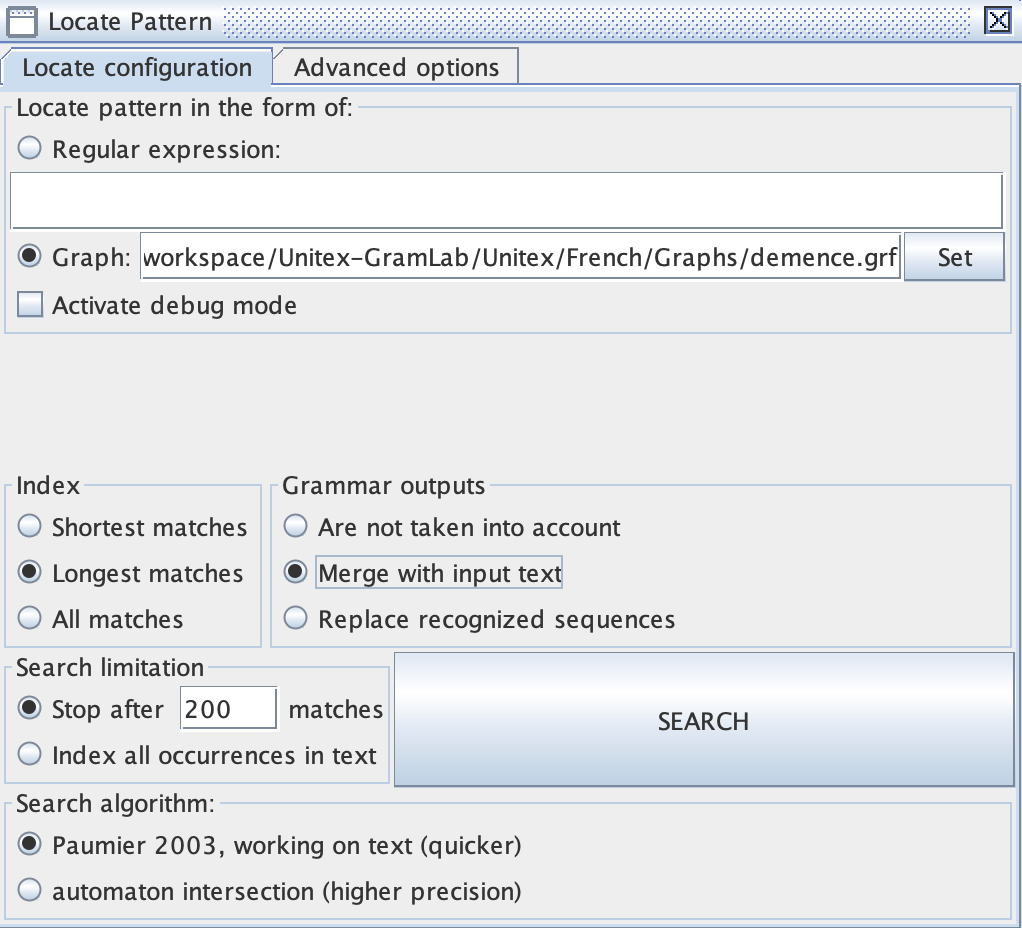
\includegraphics[width=.4\linewidth]{img/merge.png}
		\caption{Appliquer les annotations.}
		\label{fig:ling_out_TAL}
	\end{figure}
\end{frame}

\begin{frame}[allowframebreaks]
		\printbibliography
\end{frame}




\begin{frame}{Licence}
	\centering
	{\small Le contenu de cette présentation est sous licence \texttt{CC-BY-NC-SA 4.0}\\Utilisation non commerciale -- Partage dans les mêmes conditions.\\}
	\href{https://creativecommons.org/licenses/by-nc-sa/4.0/deed.fr}{\ccbyncsa}
\end{frame}

\end{document}